\documentclass[border=5pt]{standalone}
\usepackage{tikz}
\usepackage{tikz-3dplot}
\usetikzlibrary{arrows.meta, 3d, perspective, calc}
\usepackage{amsmath}
\begin{document}
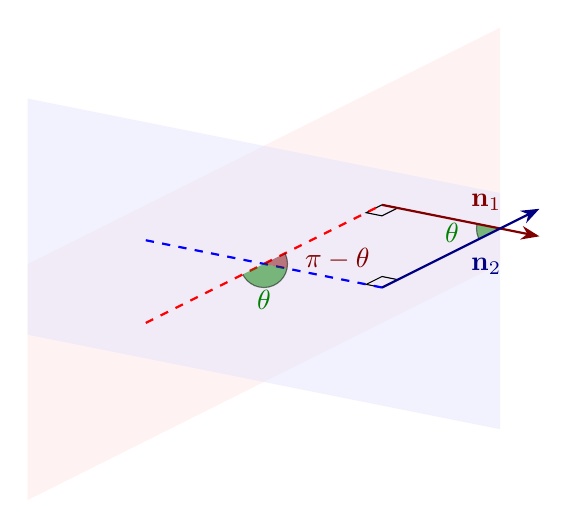
\begin{tikzpicture}[>=Stealth, x={(1cm,0.5cm)}, y={(0cm,1cm)}, z={(1cm,-0.2cm)}]

    % Planes
    \fill[red!10, opacity=0.5] (-3,0,0) -- (3,0,0) -- (3,3,0) -- (-3,3,0) -- cycle;
    \fill[blue!10, opacity=0.5] (0,0,-3) -- (0,3,-3) -- (0,3,3) -- (0,0,3) -- cycle;

    \draw[black] (1.5,1.5,0) -- (1.3,1.5,0)-- (1.3,1.5,0.2)-- (1.5,1.5,0.2)  -- cycle;

    \draw[black] (0,1.5,1.5) -- (0.2,1.5,1.5)-- (0.2,1.5,1.3)-- (0,1.5,1.3)  -- cycle;

    \draw[thick, red, dashed] (-1.5,1.5,0) -- (1.5,1.5,0);
    \draw[thick, blue, dashed] (0,1.5,-1.5) -- (0,1.5,1.5);

    \begin{scope}
        \path[clip] (0,1.5,0) -- (-1.5,1.5,0) -- (0,1.5,1.5);
        \fill[green!50!black, opacity=0.5, draw=black] (0,1.5,0) circle (3mm);
        \end{scope}
    \node[below, green!50!black] at (-0.3,1.5,0.3) {$\theta$};

    \begin{scope}
        \path[clip] (0,1.5,0) -- (1.5,1.5,0) -- (0,1.5,1.5);
        \fill[red!50!black, opacity=0.5, draw=black] (0,1.5,0) circle (3mm);
        \end{scope}
    \node[right, red!50!black] at (0.2,1.5,0.2) {$\pi-\theta$};

    \begin{scope}
        \path[clip] (1.5,1.5,1.5) -- (1.5,1.5,0) -- (0,1.5,1.5);
        \fill[green!50!black, opacity=0.5, draw=black] (1.5,1.5,1.5) circle (3mm);
        \end{scope}
    \node[left, green!50!black] at (1.3,1.5,1.3) {$\theta$};
    % Normals
    \draw[->, thick, red!50!black] (1.5,1.5,0) -- node[above right] {$\mathbf{n}_1$} (1.5,1.5,2);
    \draw[->, thick, blue!50!black] (0,1.5,1.5) -- node[below right] {$\mathbf{n}_2$} (2,1.5,1.5);
  \end{tikzpicture}
\end{document}
